\documentclass[xcolor=pdftex,dvipsnames,table,handout]{beamer}
\usetheme{Madrid}
\usepackage{color}
\usepackage{algpseudocode}

\title[Sequential Minimal Optimization]{Sequential Minimal Optimization: A Fast Algorithm for Training Support Vector Machines}
\subtitle{John C. Platt, 1998, Microsoft Research}
\author[SY Chou]{Sheng-Yen Chou}

\institute[NTHU CS]{Department of Computer Science\\ 
National Tsing Hua University}

\date{\today}

\begin{document}
\begin{frame}
  \titlepage
\end{frame}

\begin{frame}  
\frametitle{Support Vector Machine(SVM)}
\begin{center}
    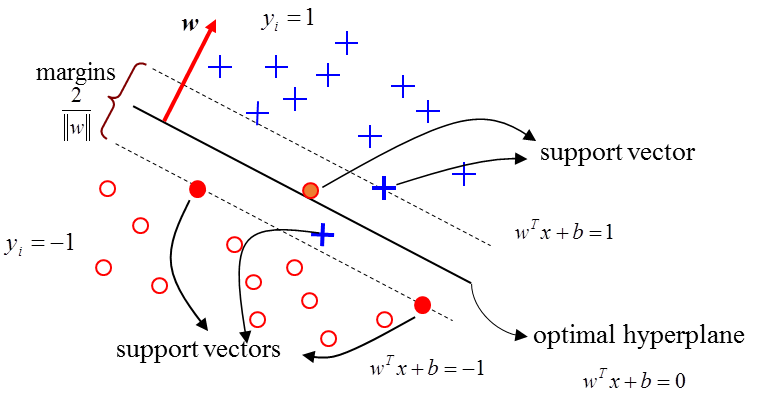
\includegraphics[width=4in]{./imgs/svm.png}
\end{center}
\end{frame}

\begin{frame}  
\frametitle{Support Vector Machine(SVM)}
In classification problem, we aim to find out a pair of parallel decision planes $w^{\top} \mathbf{x}_{+} + b_{+} \geq 1$ and $w^{\top} \mathbf{x}_{-} + b_{-} \leq -1$ such that we can separate two groups of data points $\mathbf{x}_{+}, \mathbf{x}_{-}$ perfectly and enlarge the gap $\frac{2}{||w||}$ between the nearest decision planes. 

Then we can write down the optimization problem as 

\begin{equation}
\label{eqn:einstein}
\max_{w, b} \frac{2}{||w||} \ \text{subject to} \ \mathbf{y}^{\top} \odot (w^{\top} \mathbf{x} + b) \geq 1
\end{equation}

In terms of minimization

\begin{equation}
\label{eqn:einstein}
\min_{w, b} \frac{||w||}{2} \ \text{subject to} \ \mathbf{y}^{\top} \odot (w^{\top} \mathbf{x} + b) \geq 1
\end{equation}

Where the operator $\odot$ means the element-wise product and the norm $|| \cdot ||$ is the Euclidean(L2) norm.

\end{frame}

\begin{frame}  
\frametitle{Lagrange Function}
Let $\mathbf{\alpha} \in \mathbb{R}^N, \mathbf{\alpha} > 0$ be the Lagrange multiplier, the Lagrangian function is 

$$
L(w, b, \alpha) = \frac{||w||}{2} -  (\mathbf{y}^{\top} \odot (w^{\top} \mathbf{x} + b) - 1) \mathbf{\alpha}
$$

$$
= \frac{1}{2} w^{\top} w - \sum_{i=1}^{N} \alpha_i (y_i (w^{\top} x_i + b) - 1)
$$

We aim to minimize the Lagrangian function to solve the constraint optimization problem

$$
\min_{w, b, \mathbf{\alpha}} L(w, b, \mathbf{\alpha}), \ \mathbf{\alpha} > 0
$$
\end{frame}

\begin{frame}  
\frametitle{Derive Dual Problem}
A common way to obtain the minimum of the function is letting the gradient of the function be 0.

As for variable $w$, we can derive

$$
\frac{\partial L(w, b, \mathbf{\alpha})}{\partial w} = w - \sum_{i=1}^{N} \alpha_i y_i x_i = 0 \quad \to \quad w = \sum_{i=1}^{N} \alpha_i y_i x_i
$$

As for variable $b$, we can derive

$$
\frac{\partial L(w, b, \mathbf{\alpha})}{\partial b} = \sum_{i=1}^{N} - \alpha_i y_i = 0 \quad \to \quad \sum_{i=1}^{N} \alpha_i y_i = 0
$$
\end{frame}

\begin{frame}  
\frametitle{Derive Dual Problem}

Then, we can substitute $w$ and $b$ of the Lagrangian function $L(w, b, \mathbf{\alpha})$ as 

$$
L(w, b, \mathbf{\alpha}) = \sum_{i=1}^{N} \alpha_i - \frac{1}{2} \sum_{i=1}^{N} \sum_{j=1}^{N} \alpha_i \alpha_j y_i y_j x_i^{\top} x_j
$$

Consider kernel trick, we can replace the inner product as kernel function $k(x_i, x_j) = \phi(x_i) \phi(x_j)$ with embedding function $\phi(\cdot)$

$$
L(w, b, \mathbf{\alpha}) = \sum_{i=1}^{N} \alpha_i - \frac{1}{2} \sum_{i=1}^{N} \sum_{j=1}^{N} \alpha_i \alpha_j y_i y_j k(x_i, x_j)
$$

Now, we can rewrite the optimization problem of hard-margin SVM as 

$$
\begin{tabular}{ c c c }
 $\sup_{\alpha} \sum_{i=1}^{N} \alpha_i - \frac{1}{2} \sum_{i=1}^{N} \sum_{j=1}^{N} \alpha_i \alpha_j y_i y_j k(x_i, x_j)$\\  
 $\text{subject to} \  0 \leq \alpha_i, \sum_{i=1}^{N} \alpha_i y_i= 0$\\
\end{tabular}
$$
\end{frame}

\begin{frame}  
\frametitle{Quadratic Programming}
\begin{block}{General Form of Quadratic Programming}
$$
\min_{x} g(x) = x^{\top} G x + x^{\top} c
$$

\begin{center}
\begin{tabular}
    $\text{s.t.} a_{i}^{\top} x = b_i, i \in \mathcal{E}$ \\
    $a_{i}^{\top} x \geq b_i, i \in \mathcal{I}$ \\
\end{tabular}
\end{center}

\end{block}
The optimization problem of soft-margin SVM is

$$
\begin{tabular}{ c c c }
 $\sup_{\alpha} \sum_{i=1}^{N} \alpha_i - \frac{1}{2} \sum_{i=1}^{N} \sum_{j=1}^{N} \alpha_i \alpha_j y_i y_j k(x_i, x_j)$\\  
 $\text{subject to} \ 0 \leq \alpha_i \leq C, \sum_{i=1}^{N} \alpha_i y_i= 0$\\
\end{tabular}
$$

Which satisfies quadratic programming absolutely and $C$ is the hyperparameter of soft-margin.
\end{frame}

\begin{frame}  
\frametitle{Issues of traditional ways to solve quadratic programming}
\begin{itemize}[<+->]
\item Most of methods like Gradient projection method, Newton's method... solve the whole quadratic programming in one time. However, SVM has a large matrix to solve(about $N^2$) and it would be very time consuming.

\item How about \textbf{divide-and-conquer}?
\end{itemize}
\end{frame}

\begin{frame}  
\frametitle{Divide-and-Conquer}
\begin{block}{Osuna's Theorem}
Divide the variables $\alpha_1, \alpha_2, ..., \alpha_N$ into 2 groups as $\alpha_B$ and $\alpha_H$. Fix the values of $\alpha_H$ and only update the variables of $\alpha_B$. Moving a variable that violates the optimality conditions(KKT conditions in SVM) from $\alpha_N$ to $\alpha_B$ gives a strict improvement in the cost function 
when the sub-problem is re-optimized.
\end{block}
\begin{itemize}[<+->]
\item According If we can optimize a variable that violating the KKT conditions each time, then the target function(cost function) would converge.

\item A series of works are proposed based on Osuna's Theorem, like Chunking, Osuna's algorithm... But still, the sub-problem isn't small enough.

\item SMO only solves the minimal size of sub-problem while considering KKT conditions, that is 2-variable quadratic programming.
\end{itemize}
\end{frame}

\begin{frame}  
\frametitle{Sequential Minimal Optimization(SMO)}
\begin{block}{Sequential Minimal Optimization(SMO)}
The SMO(Sequential Minimal Optimization) algorithm is proposed from the paper Sequential Minimal Optimization: A Fast Algorithm for Training Support Vector Machines in 1998 by J. Platt.
\end{block}

There are 3 steps

\begin{itemize}[<+->]
\item Step 1. Select and Update

Select 2 variables $\alpha_i, \alpha_j$ and update

\item Step 2. Box Constraint

Clip the value of $\alpha_j$ with complementary slackness

Derive the new values $\alpha_i^*, \alpha_j^*$

\item Step 3. Update Bias

Derive new bias $b^*$ from $\alpha_i^*, \alpha_j^*$
\end{itemize}
\end{frame}

\begin{frame}  
\frametitle{Step 1. Select and Update}
Denote $x_i$, $y_i$ as i-th data point and label. Let $K_{i, j} = k(x_i, x_j)$, where $k(a, b)$ is the kernel function and $f_{\phi}(x_i)$ is the prediction function.

\begin{itemize}[<+->]

\item In order to optimize the target function $L(w, b, \alpha)$, we can derive the gradient of it and let the gradient be 0.

$$
\frac{\partial L(w, b \alpha)}{\partial w} = w - \sum_{i=1}^N \alpha_i y_i x_i = 0 \to w = \sum_{i=1}^N \alpha_i y_i x_i
$$

\item In order to hold the constraint, both new variables and old variables should satisfy the constraint

$$
\sum_{i=1}^{N} \alpha_i y_i = \alpha_1 y_1 + \alpha_2 y_2 + \sum_{i=3}^{N} \alpha_i y_i = 0
$$

$$
\alpha_1^{new} y_1 + \alpha_2^{new} y_2 = \alpha_1 y_1 + \alpha_2 y_2 = - \sum_{i=3}^{N} \alpha_i y_i = \zeta
$$

\end{itemize}

\end{frame}

\begin{frame}  
\frametitle{Step 1. Select and Update}
Plug the two equations into the target function and we can derive 

$$E_i = f(x_i) - y_i, \ E_j = f(x_j) - y_j$$

$$\eta = K_{i, i} + K_{j, j} -  2 K_{i, j}$$

Then, we get a new value of $\alpha_j$

$$\alpha_j^{new} = \alpha_j + \frac{y_j (E_i - E_j)}{\eta}$$

To understand intuitively, you can see $\eta$ as \textbf{Learning Rate} and $y_j (E_i - E_j)$ as a kind of \textbf{Loss}.
\end{frame}

\begin{frame}  
\frametitle{Step 2. Box Constraint}
To satisfy the complementary slackness $\alpha_1 y_1 + \alpha_2 y_2  = \zeta, \ 0 \leq \alpha_i \leq C$, we need to \textbf{clip} the $\alpha_j^{new}$ under blue and grey area.

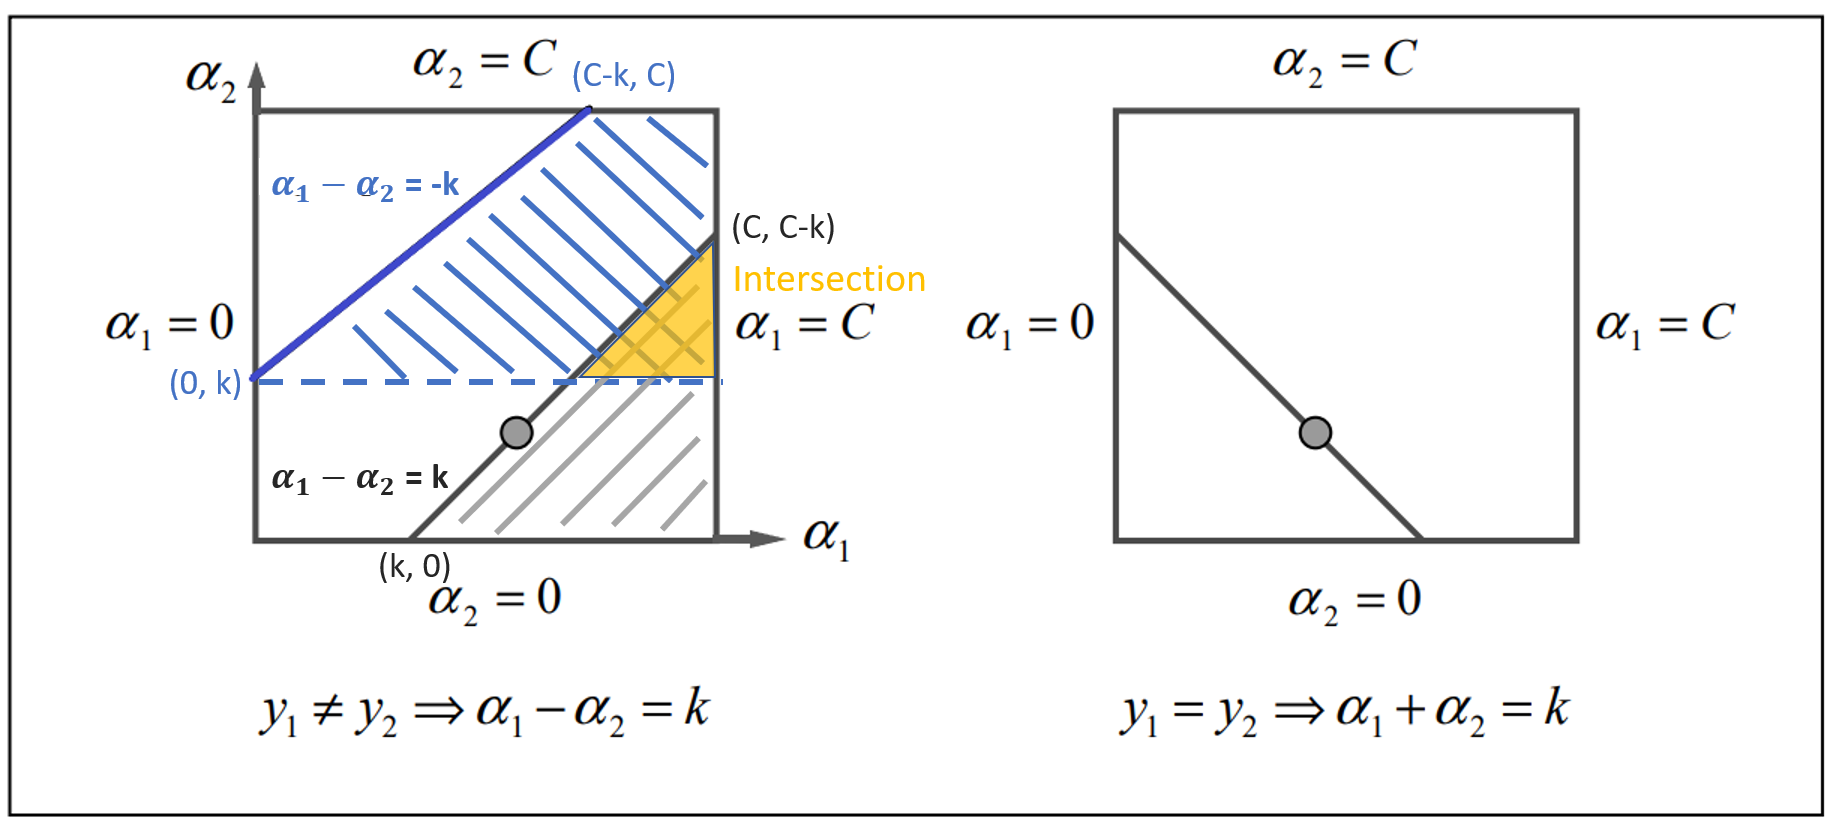
\includegraphics[width=4in]{./imgs/box.png}
\end{frame}

\begin{frame}  
\frametitle{Step 2. Box Constraint}

\begin{algorithmic}
\If{$y_i = y_j$} 
    \State $B_U = \min(C, \alpha_j + \alpha_i)$
    \State $B_L = \max(0, \alpha_j + \alpha_i - C)$
\Else
    \State $B_U = \min(C, C + \alpha_j - \alpha_i)$
    \State $B_L = \max(0, \alpha_j - \alpha_i)$
\EndIf 
\State $\alpha_j^* = CLIP(\alpha_j, B_L, B_U)$
\State $\alpha_i^* = \alpha_i + y_i y_j(\alpha_j - \alpha_j^*)$
\end{algorithmic}

% \begin{itemize}[<+->]
% \item if($y_i = y_j$):
%     \begin{itemize}[<+->]
%         \item $B_U = \min(C, \alpha_j + \alpha_i)$
%         \item $B_L = \max(0, \alpha_j + \alpha_i - C)$
%     \end{itemize}
% \item else
%     \begin{itemize}[<+->]
%         \item $B_U = \min(C, C + \alpha_j - \alpha_i)$
%         \item $B_L = \max(0, \alpha_j - \alpha_i)$
%     \end{itemize}
% \item $\alpha_j^* = CLIP(\alpha_j^{new}, B_L, B_U)$
% \item $\alpha_i^* = \alpha_i + y_i y_j(\alpha_j - \alpha_j^*)$
% \end{itemize}
\end{frame}

\begin{frame}  
\frametitle{Step 3. Update Bias}

We denote the prediction of the SVM as $f_{\phi}(x)$

$$
f_{\phi}(x_p) = w^{\top} \phi(x_p) + b = b + \sum_{i=1}^N \alpha_i y_i k(x_i, x_p)
$$

While $f_{\phi}^*(x)$ is the prediction of the SVM with new variables $\alpha_1^*$, $\alpha_2^*$, and $b^*$

$$
f_{\phi}^*(x_p) = \sum_{i=3}^N \alpha_i y_i K_{i, p} + \alpha_1^* y_1 K_{1, p} + \alpha_2^* y_2 K_{2, p} + b^* = y_p
$$
\end{frame}

\begin{frame}  
\frametitle{Step 3. Update Bias}
Thus, we can derive 3 cases

\begin{itemize}[<+->]
\item CASE 1. According to the \textbf{complementary slackness}, if $0 < \alpha_1^* < C$, the data point $x_1$ should right on the margin and $f_{\phi}^*(x_1) = y_1$. The bias derived from $\alpha_1$.

$$
b_1^* = y_1 - \sum_{i=3}^N \alpha_i y_i K_{i, 1} - \alpha_1^* y_1 K_{1, 1} - \alpha_2^* y_2 K_{2, 1}
$$

$$
= - E_1 - y_1 K_{1, 1} (\alpha_1^* - \alpha_1) - y_2 K_{2, 1} (\alpha_2^* - \alpha_2) + b
$$

\item CASE 2. If $0 < \alpha_2^* < C$, the data point $x_2$ should right on the margin and $f_{\phi}^*(x_2) = y_2$. The bias derived from $\alpha_2$.

$$
b_2^* = y_2 - \sum_{i=3}^N \alpha_i y_i K_{i, 2} - \alpha_1^* y_1 K_{1, 2} - \alpha_2^* y_2 K_{2, 2}
$$

$$
= - E_2 - y_1 K_{1, 2} (\alpha_1^* - \alpha_1) - y_2 K_{2, 2} (\alpha_2^* - \alpha_2) + b
$$
\end{itemize}
\end{frame}

\begin{frame}  
\frametitle{Step 3. Update Bias}
\begin{itemize}[<+->]
\item CASE 3. When the data point $x_i, x_j$ are both not on the margin, we choose the average of $b_1^*, b_2^*$ as the updated value.

$$
b^* = \frac{b_1^* + b_2^*}{2}
$$
\end{itemize}
\end{frame}

\begin{frame}  
\frametitle{Step 3. Update Bias}
When $0 \lt \alpha_i^* \lt C$, the data point $x_i$ is right on the margin such that $f_{\phi}(x)=y_i$.

\begin{algorithmic}
\State $b_i^* = - E_i - y_i K_{i, i} (\alpha_i^* - \alpha_i) - y_j K_{j, i} (\alpha_j^* - \alpha_j) + b$
\State $b_j^* = - E_j - y_i K_{i, j} (\alpha_i^* - \alpha_i) - y_j K_{j, j} (\alpha_j^* - \alpha_j) + b$
\If{$0 \leq \alpha_i \leq C$}
    \State $b^* = b_i^*$
\ElsIf $0 \leq \alpha_j \leq C$
    \State $b^* = b_j^*$
\Else
    \State $b^* = \frac{b_i^* + b_j^*}{2}$
\end{algorithmic}

% - $b_i^* = - E_i - y_i K_{i, i} (\alpha_i^* - \alpha_i) - y_j K_{j, i} (\alpha_j^* - \alpha_j) + b$  
% - $b_j^* = - E_j - y_i K_{i, j} (\alpha_i^* - \alpha_i) - y_j K_{j, j} (\alpha_j^* - \alpha_j) + b$

% - if($0 \leq \alpha_i \leq C$):

%     - $b^* = b_i^*$

% - else if($0 \leq \alpha_j \leq C$):

%     - $b^* = b_j^*$
    
% - else:

%   - $b^* = \frac{b_i^* + b_j^*}{2}$
\end{frame}

\begin{frame}  
\frametitle{Benchmark}
\begin{center}
    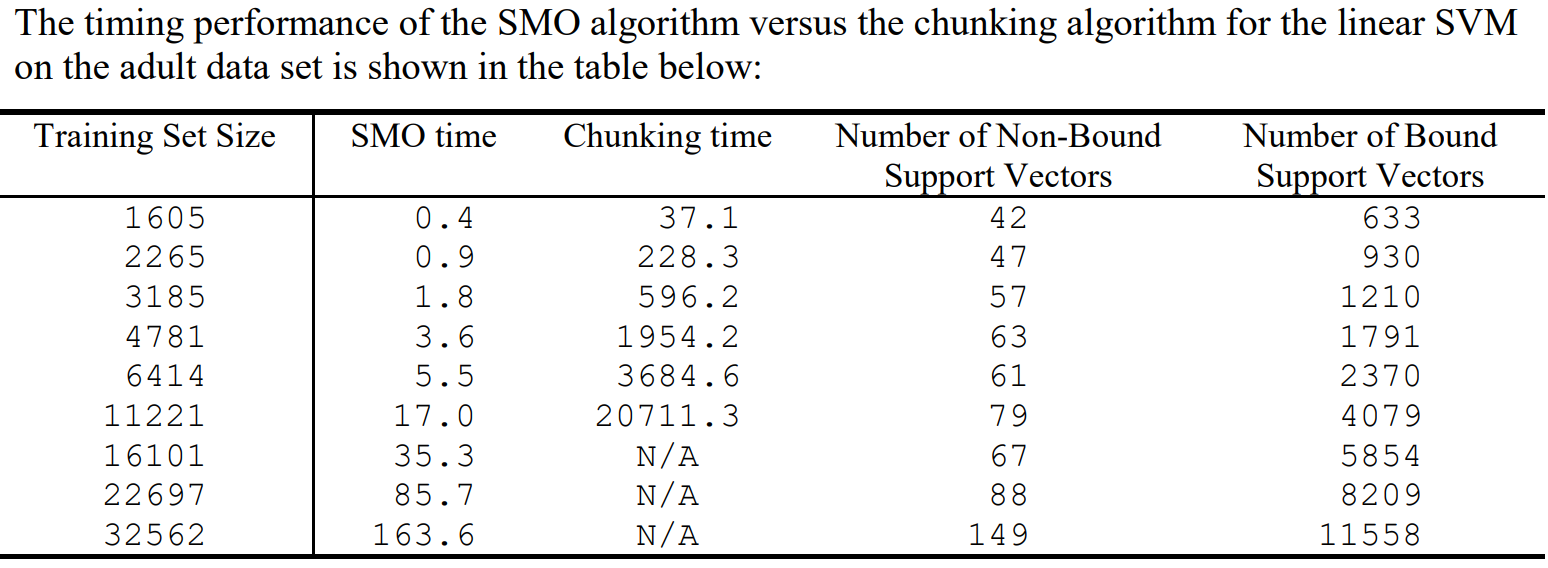
\includegraphics[width=4in]{./imgs/linear_svm.png}
    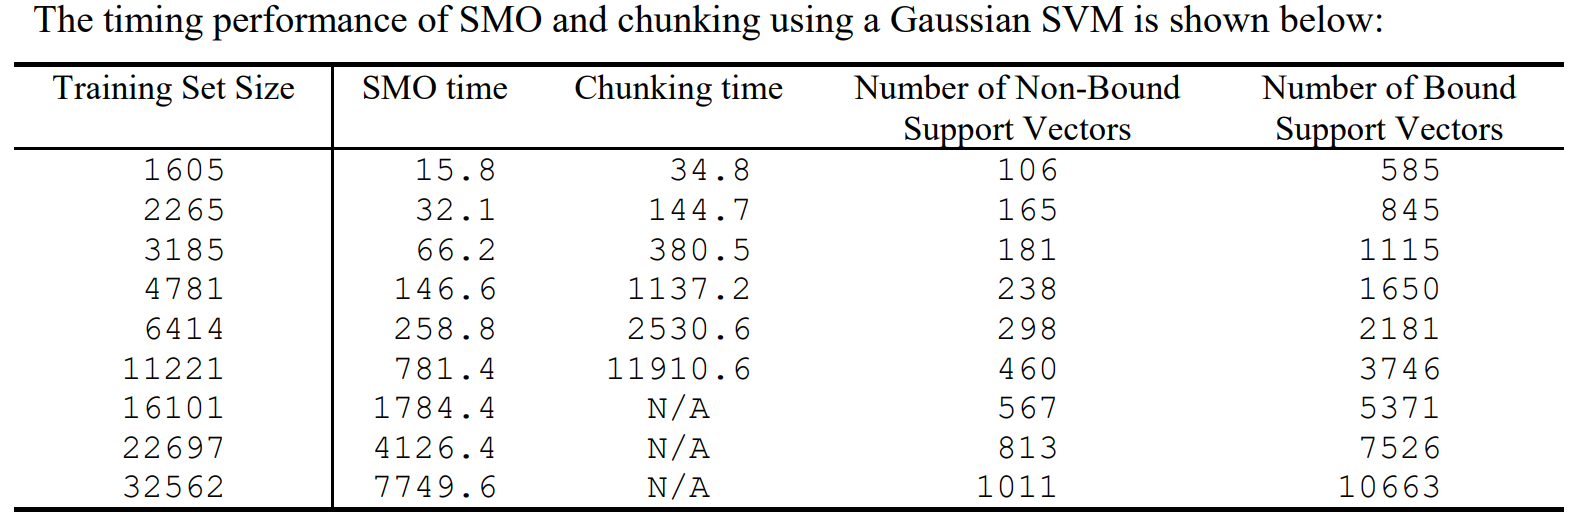
\includegraphics[width=4in]{./imgs/gaussian_svm.png}
\end{center}
\end{frame}

% \begin{frame}  
% \frametitle{Algorithm}
% 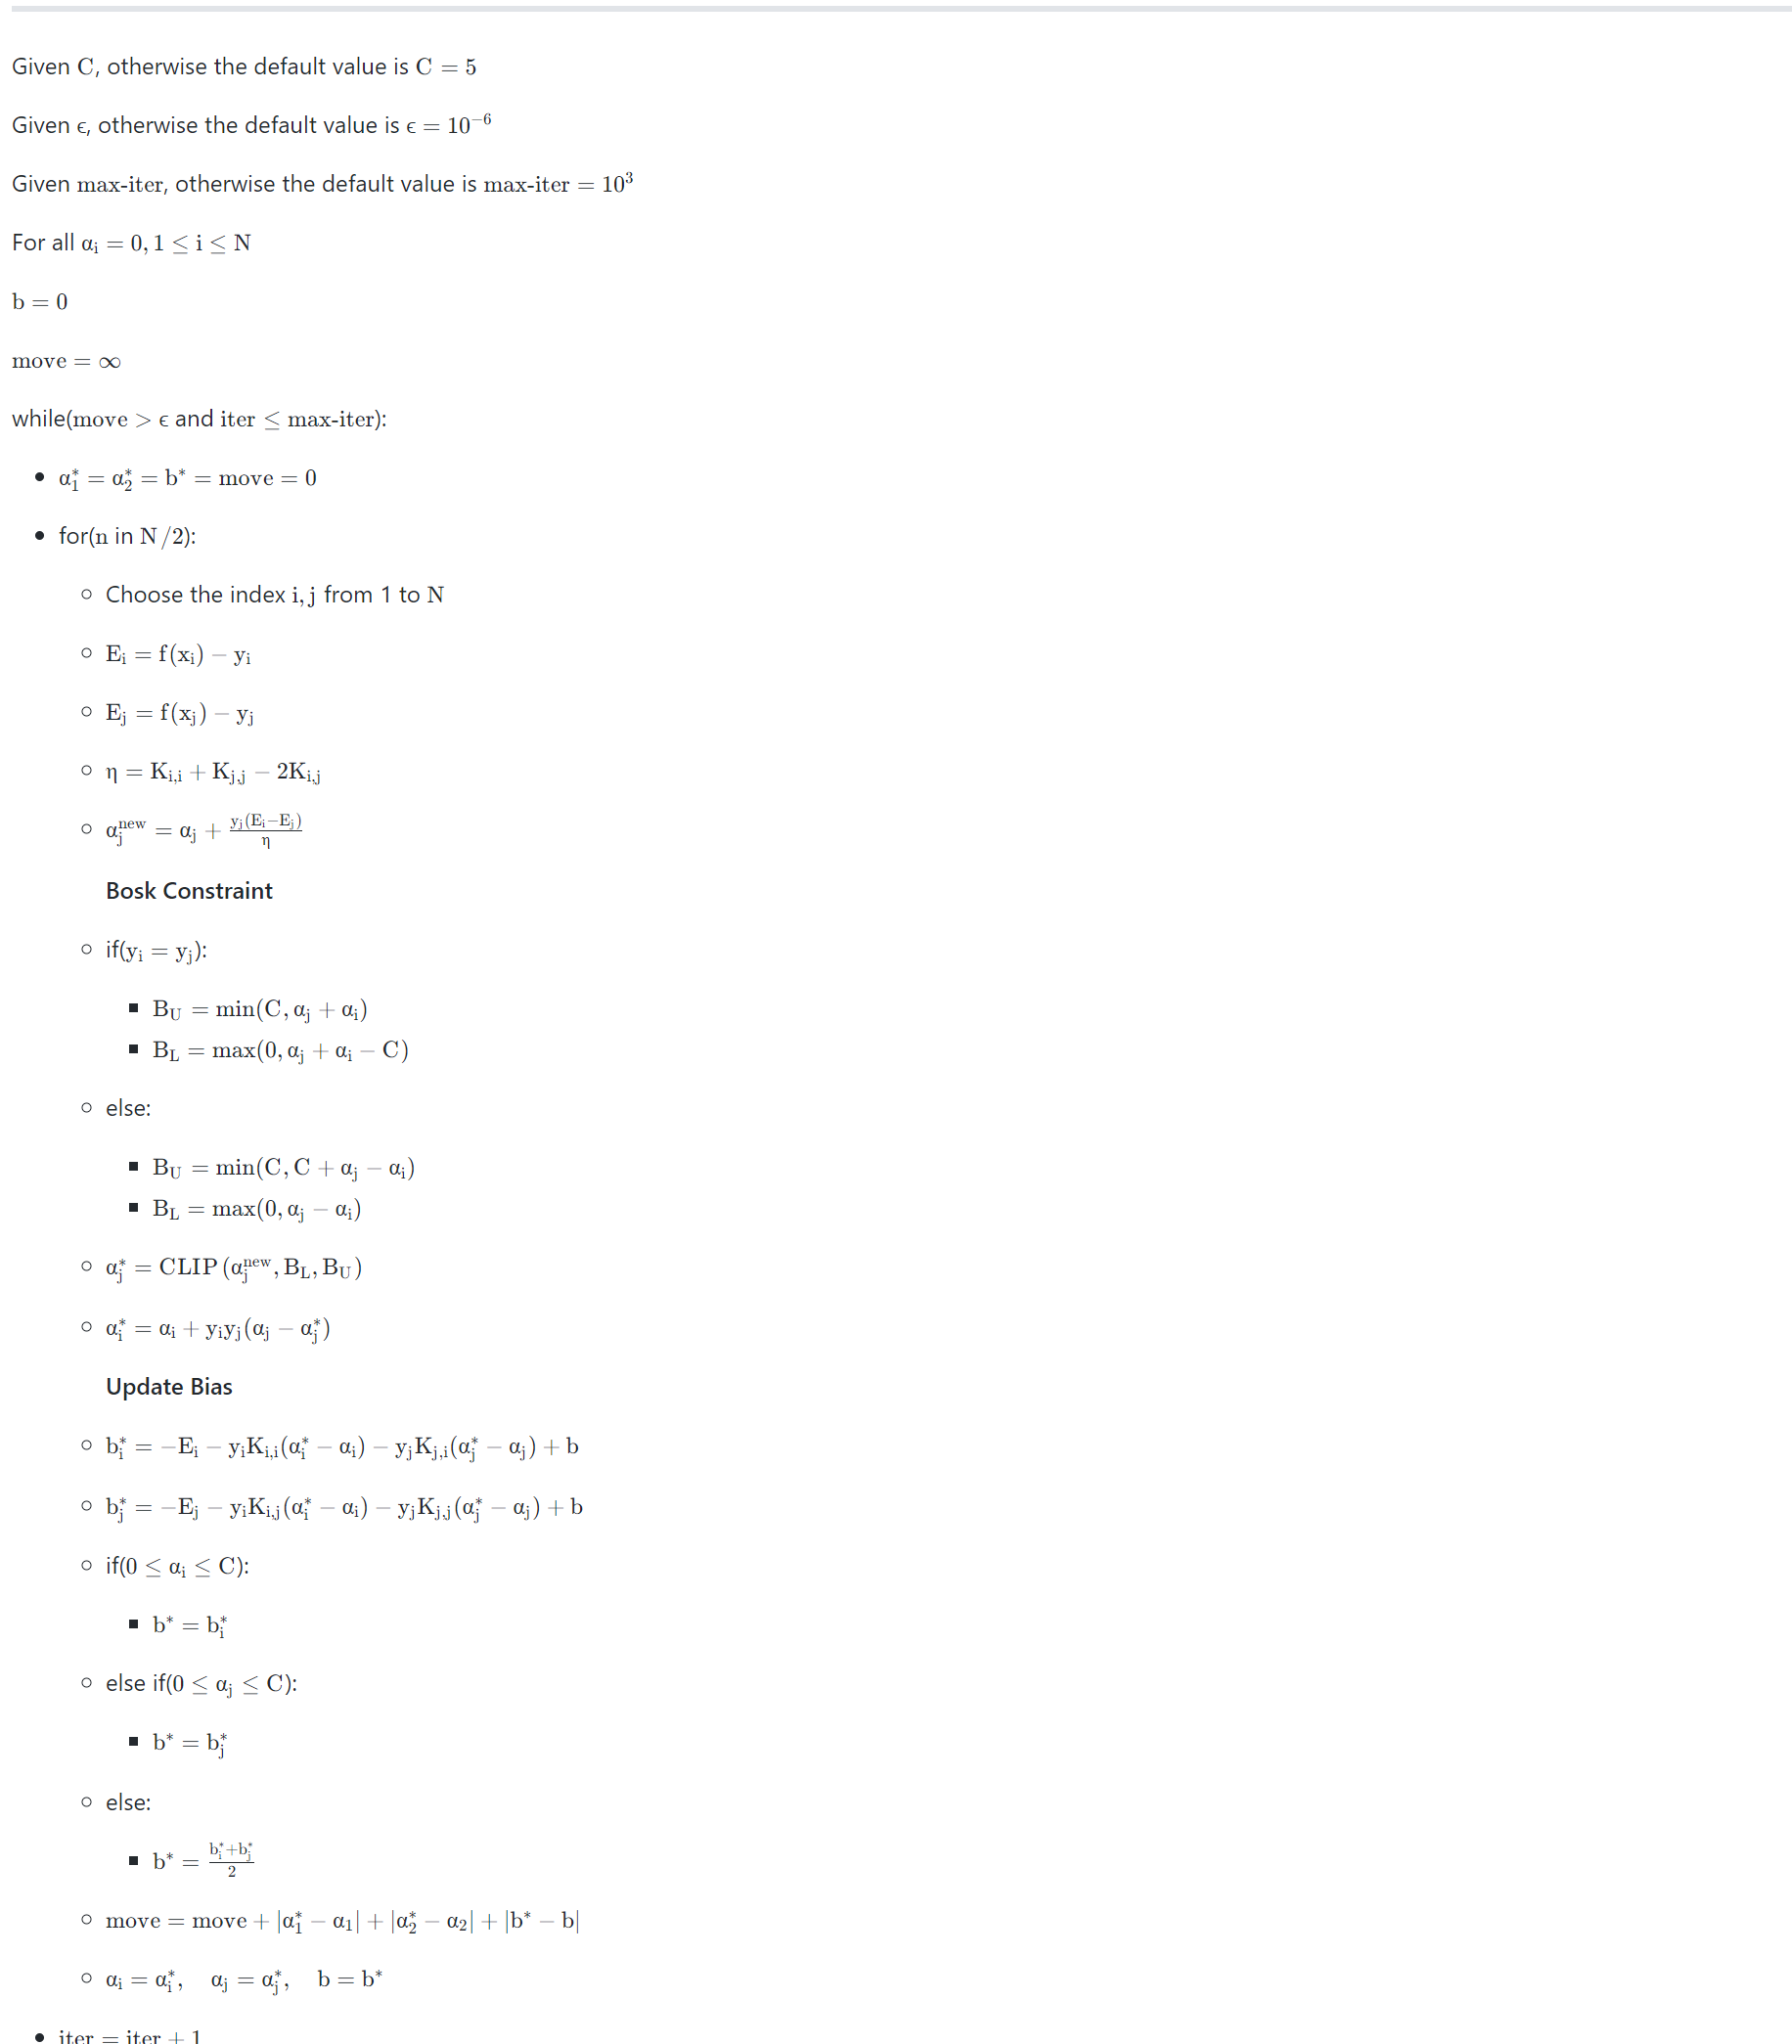
\includegraphics[width=4in]{./imgs/svm_algo.png}
% \end{frame}

\begin{frame}  
\begin{center}
    \Huge{Thanks For Listening}
\end{center}
\end{frame}

% \begin{frame}  
% \frametitle{Title of the slide}
% \begin{block}{Block of information}
% \begin{enumerate}
% \item item 1
% \item item 2
% 	\begin{enumerate}
% 	\item list 1
% 	\item list 2
% 	\end{enumerate}
% \end{enumerate}
% \end{block}

% \begin{itemize}[<+->]
% \item item 1
% \item item 2
% \item item 3
% \end{itemize}
% \end{frame}

% \begin{frame}  \frametitle{Use columns}
% \begin{columns}
% \column{2.5in}
% \begin{definition}[1.1]
% A point $x^{*}$ is a {\color{red} global minimum} of $f(x)$ if for all $y$ in the feasible set of $x$, $$f(x^{*}) \leq f(y).$$
% \end{definition}
% \begin{definition}[1.2]
% A point $x^{*}$ is a {\color{red} local minimum} of $f(x)$ in the neighborhood $N(x^{*},r)$ if for all $y \in N(x^{*},r)$, $$f(x^{*}) \leq f(y).$$
% \end{definition}
% \column{2in}
% \centering
% 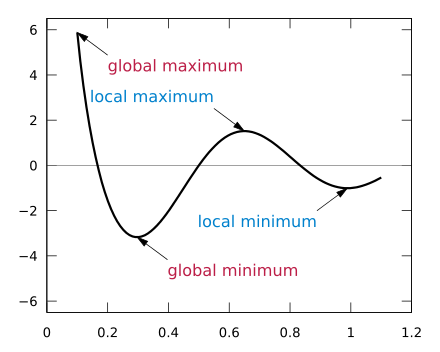
\includegraphics[width=2in]{imgs/minimum.png}
% \end{columns}
% \end{frame}

\end{document} 